\documentclass[10pt,oneside,onecolumn,openany,final]{memoir}
\setstocksize{11in}{8.5in}

\usepackage[toc,lot,lof]{multitoc}
\usepackage[top=.5in, bottom=.5in, left=.75in, right=.75in]{geometry}
\usepackage{graphicx} \graphicspath{{./images/}}
\usepackage{longtable}
\usepackage{mdwlist}
\usepackage{microtype} \DisableLigatures{encoding = *, family = *}
\usepackage{multicol}
\usepackage{textcomp}
\usepackage[normalem]{ulem}
\usepackage{wrapfig}
\usepackage{xtab}
\usepackage{enumerate}
\usepackage{phonetic}
\usepackage{bbding}
\usepackage{linearb}
\usepackage{cypriot}
\usepackage{tipa}
\usepackage{xfrac}
\usepackage{appendix}
\usepackage{xparse}
\usepackage{letltxmacro}
\usepackage{makeidx} \makeindex
\usepackage[table,dvipsnames]{xcolor}
\definecolor{offyellow}{RGB}{255,255,128}
\definecolor{links}{RGB}{200,0,50}
\usepackage{placeins}
\usepackage{floatflt}
\usepackage{anyfontsize}
\usepackage{colortbl}
\usepackage{tabularx}
\usepackage{mdframed}
\usepackage{longtable}
\usepackage{tabu}
\usepackage{afterpage}

\usepackage{caption}

%% Font
\usepackage[T1]{fontenc}
\usepackage[bitstream-charter]{mathdesign}
\usepackage{aurical}

\usepackage[colorlinks=true,linkcolor=blue,urlcolor=links,pdfstartview={XYZ null null 1.00},bookmarksdepth=2]{hyperref}
%%%%%%%%%%%%%%%%%%%%%%%%%
%%%% End of Import tion %%%%%%%%%%%
%%%%%%%%%%%%%%%%%%%%%%%%%

%%%%%%%%%%%%%%%%%%%%%%%%%%%%%%%%%%%%%%%%%%%%%%%%%%
%%%%%%%%%%%%%%%%%%%%%%%%%%%%%%%%%%%%%%%%%%%%%%%%%%
%%% Revised Commands
%%%%%%%%%%%%%%%%%%%%%%%%%%%%%%%%%%%%%%%%%%%%%%%%%%
%%%%%%%%%%%%%%%%%%%%%%%%%%%%%%%%%%%%%%%%%%%%%%%%%%
\makeatletter

%fiddles with how chapter titles are displayed
\renewcommand{\@makechapterhead}[1]{%
\vspace*{0 pt}{%
\raggedright \normalfont \fontsize{32}{32} \selectfont \bfseries%
\ifnum \value{secnumdepth}>-1%
  \if@mainmatter \vspace{-8pt} {\fontsize{20}{20} \selectfont Chapter \thechapter:}\\[8pt]%
  \fi%
\fi
\hspace{0.65cm} #1\par\nobreak\vspace{20 pt}%
}}

%makes paragraphs show up closer together
\renewcommand{\paragraph}{%
\@startsection{paragraph}{4}%
{\z@}{1.0ex \@plus 1ex \@minus 0.2ex}{-1em} % wtf is an 'ex' anyways?
{\normalfont\normalsize\bfseries}%
}

%lets multicolumn have the proper background colors as defined by rowcolors
\let\oldmc\multicolumn
\newcommand{\mcinherit}{% Activate \multicolumn inheritance
  \renewcommand{\multicolumn}[3]{%
    \oldmc{##1}{##2}{\ifodd\rownum \@oddrowcolor\else\@evenrowcolor\fi ##3}%
  }}

\makeatother

%add labels within sections, subsections, and subsubsections
\LetLtxMacro{\oldsection}{\section}
\renewcommand{\section}[1]{\oldsection{#1}\label{sec:#1}}

\LetLtxMacro{\oldsubsection}{\subsection}
\renewcommand{\subsection}[1]{\oldsubsection{#1}\label{sec:#1}}

\LetLtxMacro{\oldsubsubsection}{\subsubsection}
\renewcommand{\subsubsection}[1]{\oldsubsubsection{#1}\label{sec:#1}}

%only put chapters and sections into the TOC
\setcounter{secnumdepth}{1}
%makes a subsubsection start off indented.
\setlength{\beforesubsubsecskip}{-\beforesubsubsecskip}

%%%%%%%%%%%%%%%%%%%%%%%%%%%%%%%%%%%%%%%%%%%%%%%%%%
%%%%%%%%%%%%%%%%%%%%%%%%%%%%%%%%%%%%%%%%%%%%%%%%%%
%%% Table Formatting
%%%%%%%%%%%%%%%%%%%%%%%%%%%%%%%%%%%%%%%%%%%%%%%%%%
%%%%%%%%%%%%%%%%%%%%%%%%%%%%%%%%%%%%%%%%%%%%%%%%%%
\newcolumntype{L}[1]{>{\raggedright\let\newline\\\arraybackslash\hspace{0pt}}m{#1}} %New type of column 'L' that is ragged-right, behaves like a paragraph, and allows manual definition of width like a 'p' column.
\newcolumntype{C}[1]{>{\centering\let\newline\\\arraybackslash\hspace{0pt}}m{#1}}  %New type of column 'C' that is centered, behaves like a paragraph, and allows manual definition of width like a 'p' column.
\newcolumntype{R}[1]{>{\raggedleft\let\newline\\\arraybackslash\hspace{0pt}}m{#1}}  %New type of column 'R' that is ragged-left, behaves like a paragraph, and allows manual definition of width like a 'p' column.
\newcommand{\header}{\rowcolor{headercolor}}
%when inserted in a row, makes that row the color headercolor

%%%%%%%%%%%%%%%%%%%%%%%%%%%%%%%%%%%%%%%%%%%%%%%%%%
%%%%%%%%%%%%%%%%%%%%%%%%%%%%%%%%%%%%%%%%%%%%%%%%%%
%%% New Commands
%%%%%%%%%%%%%%%%%%%%%%%%%%%%%%%%%%%%%%%%%%%%%%%%%%
%%%%%%%%%%%%%%%%%%%%%%%%%%%%%%%%%%%%%%%%%%%%%%%%%%

%%%%%%%%%%%%%%%%%%%%%%%%
%%Basic Formatting
%%%%%%%%%%%%%%%%%%%%%%%%
\newcommand{\originallineskip}{\baselineskip}
 %A command that is equal to the original \baselineskip of the doc, in case we change it for a section and want to change it back later
\newcommand{\ability}[2]{\smallskip
 \textbf{#1} #2} 
%The \ability{#1}{#2} command from legacy-source. Should rarely be directly used, changes to this will cascade into other new commands that use its functionality
\newcommand{\shortability}[2]{\noindent\textbf{#1} #2\\}
%A specialized version of the \ability command
\newcommand{\itemspace}{\setlength{\itemsep}{-1mm}\setlength{\topsep}{-1mm} }
%A command from legacy-source for compatabilty
\newcommand{\listone}{\begin{list}{$\bullet$}{\itemspace}}
\newcommand{\listtwo}{\begin{list}{$\triangleright$}{\itemspace}}
%A type of list from legacy sorce
\newcommand{\listnum}{\begin{list}{\textbf{\arabic{counter}}:}{\usecounter{counter}}}
\newcommand{\spell}[1]{\emph{\MakeLowercase{#1}}}
%makes spell name lowercase italics.
\setlength{\parindent}{0pt}

\newcommand{\half}[0]{\ensuremath{\sfrac{1}{2}} }
\newcommand{\third}[0]{\ensuremath{\sfrac{1}{3}} }
\newcommand{\fourth}[0]{\ensuremath{\sfrac{1}{4}} }

%%%%%%%%%%%%%%%%%%%%%%%%
%%Logic
%%%%%%%%%%%%%%%%%%%%%%%%
\newcommand{\testempty}{\empty}
\newcommand{\isempty}{\empty}
%Two commands that can be compared to one another for \ifx logic tests. \isempty should never be changed. If \testempty holds a value of anything but empty, the test should return false.
\newcounter{counter}

%%%%%%%%%%%%%%%%%%%%%%%%
%%Colors
%%%%%%%%%%%%%%%%%%%%%%%%
\colorlet{colorone}{white}
\colorlet{colortwo}{gray!15}
\colorlet{headercolor}{gray!50}
\colorlet{tablecolorone}{gray!40}
\colorlet{tablecolortwo}{gray!20}

%%%%%%%%%%%%%%%%%%%%%%%%
%%Sectioning
%%%%%%%%%%%%%%%%%%%%%%%%
\newcommand{\classentry}[1]{\newpage \section{#1} \label{class:#1} \renewcommand{\class}{#1} \index{#1 (class)} \renewcommand{\testempty}{\isempty}}
%Starts a new page, creates a section with the name of the class (#1), sets \class to be the name of the class, indexes the class.
\newcommand{\raceentry}[1]{\subsection{#1} \label{race:#1} \renewcommand{\race}{#1}}
%\newcommand{\raceentry}[1]{\oldsection{#1}\index{#1 (race)}\label{race:#1}}

\newcommand{\Requirements}{\oldsubsubsection*{Requirements}}

\newcommand{\Basics}{\oldsubsubsection*{Basics}}

\newcommand{\ClassFeatures}{\oldsubsubsection*{Class Features}}

\newcommand{\skillentry}[2]{\oldsubsection[#1]{#1 #2}\index{#1 (skill)}\label{skill:#1}}

%%%%%%%%%%%%%%%%%%%%%%%%
%%Race Chapter
%%%%%%%%%%%%%%%%%%%%%%%%
\newcommand{\race}{placeholder}

%%%%%%%%%%%%%%%%%%%%%%%%
%%Class Chapter
%%%%%%%%%%%%%%%%%%%%%%%%
\newcommand{\class}{placeholder}
%Holds the classes name, as defined by \classentry

\newcommand{\quot}[1]{
	\vspace{-8pt}
	\noindent\emph{#1}\medskip}
%Displays a flavor quote.}

\newenvironment{classpreamble}{
\renewcommand\tabularxcolumn[1]{m{##1}}
\center
\rowcolors{1}{colorone}{colortwo}
\tabularx{\textwidth}{X}
}{
\endtabularx
\endcenter
\renewcommand\tabularxcolumn[1]{p{##1}}
}

\newcommand{\desc}[1]{  #1 \\}
\newcommand{\playingaclass}[1]{\ability{Playing a \class :}{#1}\\}
\newcommand{\hitdie}[1]{\ability{Hit Die:}{#1}\\}
\newcommand{\alignment}[1]{\ability{Alignment:}{#1}\\}
\newcommand{\races}[1]{\ability{Races:}{#1}\\}
\newcommand{\startinggold}[1]{\ability{Starting Gold:}{#1}\\}
\newcommand{\startingage}[1]{\ability{Starting Age:}{#1}\\}  
\newcommand{\skillpoints}[1]{\ability{Skill Points per Level:}{#1 + Intelligence Bonus}\\}
\newcommand{\classskills}[1]{\ability{Class Skills:}{The {\class}'s class skills (and the key ability for each skill) are #1}\\}

\newcommand{\startclassfeatures}{
 \smallskip\noindent All of the following are class features of the \class ~class.}
%place before actual class features entries.

\newcommand{\proficiencies}[1]{
 \ability{Weapon and Armor Proficiencies:}{The \class ~is proficient with #1}}
%Displays proficiencies with minimal input, implimentation looks like \proficiencies{the proficiencies}

\newcommand{\classfeature}[2]{
  \ability{#1}{#2}}
%No functional difference from \ability currently

%%%%Class Table Commands

\newcommand{\gbab}{\empty}
\newcommand{\mbab}{\empty}
\newcommand{\fort}{\empty}
\newcommand{\refl}{\empty}
\newcommand{\will}{\empty}
%Creates new commands for use in \ifx statements for formatting purposes.

\newcommand{\goodbab}{\renewcommand{\gbab}{\empty}\renewcommand{\mbab}{a}}
\newcommand{\modebab}{\renewcommand{\gbab}{a}\renewcommand{\mbab}{\empty}}
\newcommand{\poorbab}{\renewcommand{\gbab}{a}\renewcommand{\mbab}{a}}
%A set of commands to tell LaTeX what BAB progression the class has. Only one should be called per class.

\newcommand{\goodfor}{\renewcommand{\fort}{\empty}}
\newcommand{\poorfor}{\renewcommand{\fort}{a}}
%A set of commands to tell LaTeX what Fortitude progression the class has. Only one should be called per class.

\newcommand{\goodref}{\renewcommand{\refl}{\empty}}
\newcommand{\poorref}{\renewcommand{\refl}{a}}
%A set of commands to tell LaTeX what Reflex progression the class has. Only one should be called per class.

\newcommand{\goodwil}{\renewcommand{\will}{\empty}}
\newcommand{\poorwil}{\renewcommand{\will}{a}}
%A set of commands to tell LaTeX what Will progression the class has. Only one should be called per class.

\newenvironment{classtable}[1]
{
\table[htb]
\center
\rowcolors{1}{colorone}{colortwo}
\tabularx{\textwidth}{p{.275in}lp{0.275in}p{0.275in}p{0.275in}Xllll}
\rowcolor{headercolor} Level & Base Attack & Fort. & Ref. & Will & Special #1\\
}{
\endtabularx
\endcenter
\endtable
}
%A a new environment that sets up the class tables. Include the \level commands between \begin{classtable}.

\newenvironment{minorcastingclasstable}
{
\table[htb]
\center
\rowcolors{1}{colorone}{colortwo}
\tabularx{\textwidth}{p{.275in}lp{0.275in}p{0.275in}p{0.275in}Xccccccc}
\rowcolor{headercolor} & & & & & &\multicolumn{7}{c}{Spells Per Day (By Level)} \\
\rowcolor{headercolor} Level & Base Attack & Fort. & Ref. & Will & Special &0&1&2&3&4&5&6\\
}{
\endtabularx
\endcenter
\endtable
}
%A a new environment similar to classtable, but with columns for a minor (zero through six) spell slot progression.

\newenvironment{fullcastingclasstable}
{
\table[htb]
\center
\rowcolors{1}{colorone}{colortwo}
\tabularx{\textwidth}{p{.275in}lp{0.275in}p{0.275in}p{0.275in}Xcccccccccc}
\rowcolor{headercolor} & & & & & &\multicolumn{10}{c}{Spells Per Day (By Level)} \\
\rowcolor{headercolor} Level & Base Attack & Fort. & Ref. & Will & Special &0&1&2&3&4&5&6&7&8&9\\
}{
\endtabularx
\endcenter
\endtable
}
%Another environment for class tables, this one for full (0 through 9) spell slot progression.

\newcommand{\levelone}[1]{
1st  & \ifx\gbab\isempty +1 \else\ifx\mbab\isempty +0 \else +0 \fi \fi
	 & \ifx\fort\isempty +2 \else +0 \fi
	 & \ifx\refl\isempty +2 \else +0 \fi
	 & \ifx\will\isempty +2 \else +0 \fi
	 & #1 \\}
%A command that declares a table row within the class feature table.

\newcommand{\leveltwo}[1]{
2nd  & \ifx\gbab\isempty +2 \else\ifx\mbab\isempty +1 \else +1 \fi \fi
	 & \ifx\fort\isempty +3 \else +0 \fi
	 & \ifx\refl\isempty +3 \else +0 \fi
	 & \ifx\will\isempty +3 \else +0 \fi
	 & #1 \\}
%A command that declares a table row within the class feature table.

\newcommand{\levelthree}[1]{
3rd  & \ifx\gbab\isempty +3 \else\ifx\mbab\isempty +2 \else +1 \fi \fi
	 & \ifx\fort\isempty +3 \else +1 \fi
	 & \ifx\refl\isempty +3 \else +1 \fi
	 & \ifx\will\isempty +3 \else +1 \fi
	 & #1 \\}
%A command that declares a table row within the class feature table.

\newcommand{\levelfour}[1]{
4th  & \ifx\gbab\isempty +4 \else\ifx\mbab\isempty +3 \else +2 \fi \fi
	 & \ifx\fort\isempty +4 \else +1 \fi
	 & \ifx\refl\isempty +4 \else +1 \fi
	 & \ifx\will\isempty +4 \else +1 \fi
	 & #1 \\}
%A command that declares a table row within the class feature table.

\newcommand{\levelfive}[1]{
5th  & \ifx\gbab\isempty +5 \else\ifx\mbab\isempty +3 \else +2 \fi \fi
	 & \ifx\fort\isempty +4 \else +1 \fi
	 & \ifx\refl\isempty +4 \else +1 \fi
	 & \ifx\will\isempty +4 \else +1 \fi
	 & #1 \\}
%A command that declares a table row within the class feature table.
	 
\newcommand{\levelsix}[1]{
6th  & \ifx\gbab\isempty +6/+1 \else\ifx\mbab\isempty +4 \else +3 \fi \fi
	 & \ifx\fort\isempty +5 \else +2 \fi
	 & \ifx\refl\isempty +5 \else +2 \fi
	 & \ifx\will\isempty +5 \else +2 \fi
	 & #1 \\}
%A command that declares a table row within the class feature table.

\newcommand{\levelseven}[1]{
7th  & \ifx\gbab\isempty +7/+2 \else\ifx\mbab\isempty +5 \else +3 \fi \fi
	 & \ifx\fort\isempty +5 \else +2 \fi
	 & \ifx\refl\isempty +5 \else +2 \fi
	 & \ifx\will\isempty +5 \else +2 \fi
	 & #1 \\}
%A command that declares a table row within the class feature table.
	 
\newcommand{\leveleight}[1]{
8th  & \ifx\gbab\isempty +8/+3 \else\ifx\mbab\isempty +6/+1 \else +4 \fi \fi
	 & \ifx\fort\isempty +6 \else +2 \fi
	 & \ifx\refl\isempty +6 \else +2 \fi
	 & \ifx\will\isempty +6 \else +2 \fi
	 & #1 \\}
%A command that declares a table row within the class feature table.
	 
\newcommand{\levelnine}[1]{
9th  & \ifx\gbab\isempty +9/+4 \else\ifx\mbab\isempty +6/+1 \else +4 \fi \fi
	 & \ifx\fort\isempty +6 \else +3 \fi
	 & \ifx\refl\isempty +6 \else +3 \fi
	 & \ifx\will\isempty +6 \else +3 \fi
	 & #1 \\}
%A command that declares a table row within the class feature table.
	 
\newcommand{\levelten}[1]{
10th & \ifx\gbab\isempty +10/+5 \else\ifx\mbab\isempty +7/+2 \else +5 \fi \fi
	 & \ifx\fort\isempty +7 \else +3 \fi
	 & \ifx\refl\isempty +7 \else +3 \fi
	 & \ifx\will\isempty +7 \else +3 \fi
	 & #1 \\}
%A command that declares a table row within the class feature table.
	 
\newcommand{\leveleleven}[1]{
11th & \ifx\gbab\isempty +11/+6/+6 \else\ifx\mbab\isempty +8/+3 \else +5 \fi \fi
	 & \ifx\fort\isempty +7 \else +3 \fi
	 & \ifx\refl\isempty +7 \else +3 \fi
	 & \ifx\will\isempty +7 \else +3 \fi
	 & #1 \\}
%A command that declares a table row within the class feature table.
	 
\newcommand{\leveltwelve}[1]{
12th & \ifx\gbab\isempty +12/+7/+7 \else\ifx\mbab\isempty +9/+4 \else +6/+1 \fi \fi
	 & \ifx\fort\isempty +8 \else +4 \fi
	 & \ifx\refl\isempty +8 \else +4 \fi
	 & \ifx\will\isempty +8 \else +4 \fi
	 & #1 \\}
%A command that declares a table row within the class feature table.
	 
\newcommand{\levelthirteen}[1]{
13th & \ifx\gbab\isempty +13/+8/+8 \else\ifx\mbab\isempty +9/+4 \else +6/+1 \fi \fi
	 & \ifx\fort\isempty +8 \else +4 \fi
	 & \ifx\refl\isempty +8 \else +4 \fi
	 & \ifx\will\isempty +8 \else +4 \fi
	 & #1 \\}
%A command that declares a table row within the class feature table.
	 
\newcommand{\levelfourteen}[1]{
14th & \ifx\gbab\isempty +14/+9/+9 \else\ifx\mbab\isempty +10/+5 \else +7/+2 \fi \fi
	 & \ifx\fort\isempty +9 \else +4 \fi
	 & \ifx\refl\isempty +9 \else +4 \fi
	 & \ifx\will\isempty +9 \else +4 \fi
	 & #1 \\}
%A command that declares a table row within the class feature table.
	 
\newcommand{\levelfifteen}[1]{
15th & \ifx\gbab\isempty +15/+10/+10 \else\ifx\mbab\isempty +11/+6/+6 \else +7/+2 \fi \fi
	 & \ifx\fort\isempty +9 \else +5 \fi
	 & \ifx\refl\isempty +9 \else +5 \fi
	 & \ifx\will\isempty +9 \else +5 \fi
	 & #1 \\}
%A command that declares a table row within the class feature table.
	 
\newcommand{\levelsixteen}[1]{
16th & \ifx\gbab\isempty +16/+11/+11/+11 \else\ifx\mbab\isempty +12/+7/+7 \else +8/+3 \fi \fi
	 & \ifx\fort\isempty +10 \else +5 \fi
	 & \ifx\refl\isempty +10 \else +5 \fi
	 & \ifx\will\isempty +10 \else +5 \fi
	 & #1 \\}
%A command that declares a table row within the class feature table.
	 
\newcommand{\levelseventeen}[1]{
17th & \ifx\gbab\isempty +17/+12/+12/+12 \else\ifx\mbab\isempty +12/+7/+7 \else +8/+3 \fi \fi
	 & \ifx\fort\isempty +10 \else +5 \fi
	 & \ifx\refl\isempty +10 \else +5 \fi
	 & \ifx\will\isempty +10 \else +5 \fi
	 & #1 \\}
%A command that declares a table row within the class feature table.
	 
\newcommand{\leveleighteen}[1]{
18th & \ifx\gbab\isempty +18/+13/+13/+13 \else\ifx\mbab\isempty +13/+8/+8 \else +9/+4 \fi \fi
	 & \ifx\fort\isempty +11 \else +6 \fi
	 & \ifx\refl\isempty +11 \else +6 \fi
	 & \ifx\will\isempty +11 \else +6 \fi
	 & #1 \\}
%A command that declares a table row within the class feature table.
	 
\newcommand{\levelnineteen}[1]{
19th & \ifx\gbab\isempty +19/+14/+14/+14 \else\ifx\mbab\isempty +14/+9/+9 \else +9/+4 \fi \fi
	 & \ifx\fort\isempty +11 \else +6 \fi
	 & \ifx\refl\isempty +11 \else +6 \fi
	 & \ifx\will\isempty +11 \else +6 \fi
	 & #1 \\}
%A command that declares a table row within the class feature table.
	 
\newcommand{\leveltwenty}[1]{
20th & \ifx\gbab\isempty +20/+15/+15/+15 \else\ifx\mbab\isempty +15/+10/+10 \else +10/+5 \fi \fi
	 & \ifx\fort\isempty +12 \else +6 \fi
	 & \ifx\refl\isempty +12 \else +6 \fi
	 & \ifx\will\isempty +12 \else +6 \fi
	 & #1 \\}
%A command that declares a table row within the class feature table.

\newmdenv[hidealllines=true,backgroundcolor=gray!20]{optionbox}

\newcommand{\option}[1]{
  \renewmdenv[hidealllines=true,backgroundcolor=colorone]{optionbox}
   \begin{optionbox}\noindent{#1}\end{optionbox}
   ~\\*
}

\newenvironment{optional}{
\colorlet{colortwo}{white}
\colorlet{colorone}{gray!15}
}


%%%%%%%%%%%%%%%%%%%%%%%%
%%Unsorted Commands
%%%%%%%%%%%%%%%%%%%%%%%%
\newcommand{\tagline}[1]{\vspace{-6pt} \textit{#1} \medskip}

\newcommand{\gameterm}[1]{#1\index{#1}}

\NewDocumentCommand\featentry{m+g}{%
  \IfNoValueTF{#2}
    {\oldsubsubsection[#1]{#1 [General]}\label{feat:#1}}%no second arg, general feat
    {\oldsubsubsection[#1]{#1 [#2]}\label{feat:#1}}%second arg, special type of feat
}

\newcommand{\spellentry}[1]{\oldsubsubsection{#1}\label{spell:#1}}

\NewDocumentCommand\linkrace{m+g}{%
  \IfNoValueTF{#2}
    {\hyperref[race:#1]{#1}}%no second arg, display is same as link
    {\hyperref[race:#1]{#2}}%second arg, link to first and display second
}
\NewDocumentCommand\linkclass{m+g}{%
  \IfNoValueTF{#2}
    {\hyperref[class:#1]{#1}}%no second arg, display is same as link
    {\hyperref[class:#1]{#2}}%second arg, link to first and display second
}
\NewDocumentCommand\linkskill{m+g}{%
  \IfNoValueTF{#2}
    {\hyperref[skill:#1]{#1}}%no second arg, display is same as link
    {\hyperref[skill:#1]{#2}}%second arg, link to first and display second
}
\NewDocumentCommand\linkfeat{m+g}{%
  \IfNoValueTF{#2}
    {\hyperref[feat:#1]{#1}}%no second arg, display is same as link
    {\hyperref[feat:#1]{#2}}%second arg, link to first and display second
}
\NewDocumentCommand\linkspell{m+g}{%
  \IfNoValueTF{#2}
    {\hyperref[spell:#1]{#1}}%no second arg, display is same as link
    {\hyperref[spell:#1]{#2}}%second arg, link to first and display second
}
\NewDocumentCommand\linkcondition{m+g}{%
  \IfNoValueTF{#2}
    {\hyperref[condition:#1]{#1}}%no second arg, display is same as link
    {\hyperref[condition:#1]{#2}}%second arg, link to first and display second
}
\NewDocumentCommand\linkability{m+g}{%
  \IfNoValueTF{#2}
    {\hyperref[ability:#1]{#1}}%no second arg, display is same as link
    {\hyperref[ability:#1]{#2}}%second arg, link to first and display second
}
\NewDocumentCommand\linksec{m+g}{%
  \IfNoValueTF{#2}
    {\hyperref[sec:#1]{#1}}%no second arg, display is same as link
    {\hyperref[sec:#1]{#2}}%second arg, link to first and display second
}

\begin{document}

%%%%%%%%%%%%%%%%%%%%%%%%%%%%%%%%%%%%%%%%%%%%%%%%%%
%%%%%%%%%%%%%%%%%%%%%%%%%%%%%%%%%%%%%%%%%%%%%%%%%%
%%% Title Page
%%%%%%%%%%%%%%%%%%%%%%%%%%%%%%%%%%%%%%%%%%%%%%%%%%
%%%%%%%%%%%%%%%%%%%%%%%%%%%%%%%%%%%%%%%%%%%%%%%%%%
\thispagestyle{empty}
\begin{center}
\textsc{\Large}\\[0.25cm]
\rule{\linewidth}{0.5mm} \\[0.70cm]
\fontsize{30}{30} \selectfont Tome Reference Document\\[.30cm]
\fontsize{16}{18} \selectfont \guillemotleft{} For that game we all known and love \guillemotright{}\\
\rule{\linewidth}{0.5mm} \\[0.6cm]
%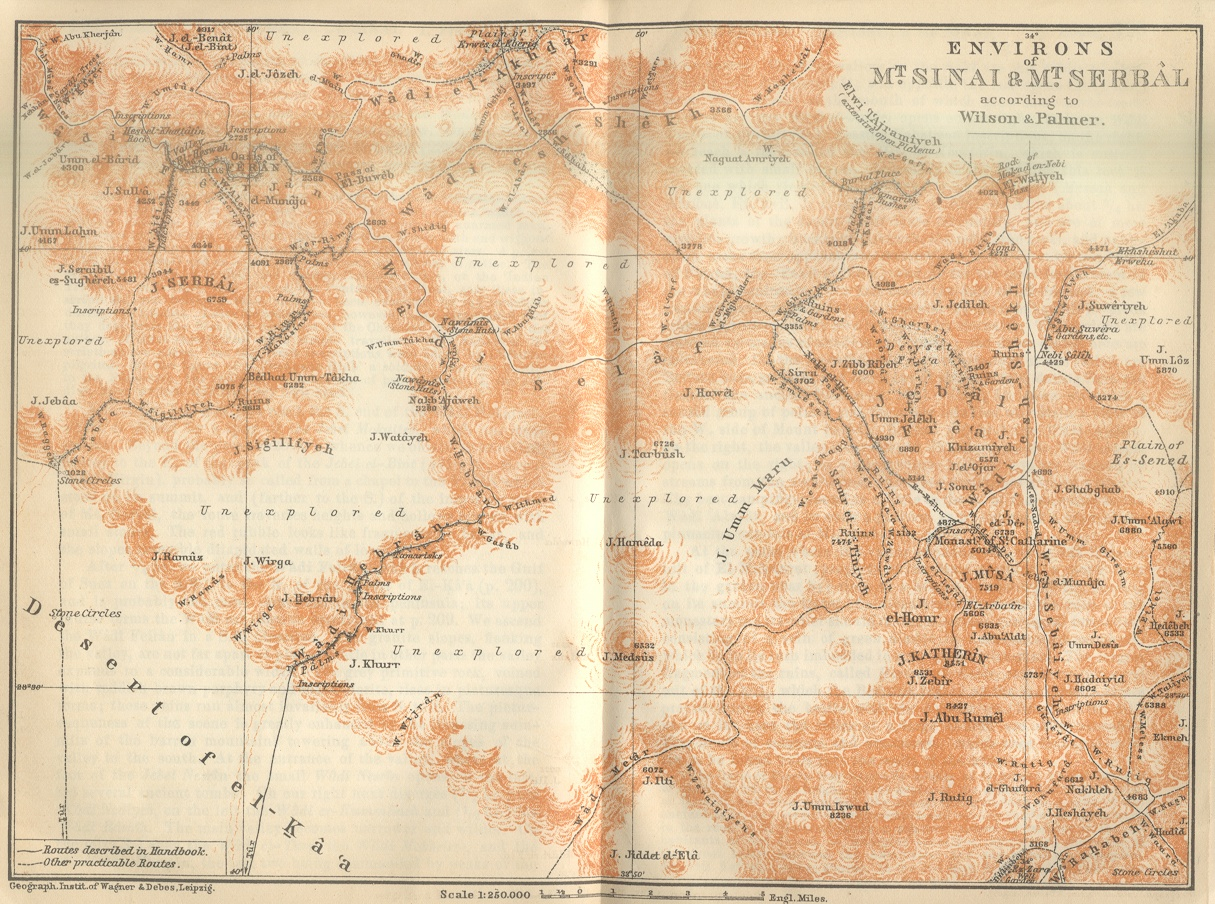
\includegraphics[clip,trim=5cm 2cm 9cm 1cm,width=\linewidth]{OldBookArt--MapImages-173.jpg}
\vfill
{\large \textit{This material is Open Game Content, and is licensed for public use under the terms of the Open Game License v1.0a.}\\
\today}
\end{center}

\pagebreak
\sffamily
\pagestyle{plain}
\raggedbottom

%%%%%%%%%%%%%%%%%%%%%%%%%%%%%%%%%%%%%%%%%%%%%%%%%%
%%%%%%%%%%%%%%%%%%%%%%%%%%%%%%%%%%%%%%%%%%%%%%%%%%
%%% Table of Contents
%%%%%%%%%%%%%%%%%%%%%%%%%%%%%%%%%%%%%%%%%%%%%%%%%%
%%%%%%%%%%%%%%%%%%%%%%%%%%%%%%%%%%%%%%%%%%%%%%%%%%
\renewcommand{\contentsname}{Table of Contents}
\setcounter{tocdepth}{1}
\tableofcontents

%%%%%%%%%%%%%%%%%%%%%%%%%%%%%%%%%%%%%%%%%%%%%%%%%%
%%%%%%%%%%%%%%%%%%%%%%%%%%%%%%%%%%%%%%%%%%%%%%%%%%
%%% Main Content
%%%%%%%%%%%%%%%%%%%%%%%%%%%%%%%%%%%%%%%%%%%%%%%%%%
%%%%%%%%%%%%%%%%%%%%%%%%%%%%%%%%%%%%%%%%%%%%%%%%%%

%% Primary Chapters Here

\clearpage

\chapter{Goods and Services}
\section{The Three Economies}
foo
\section{Armor}
foo
\section{Weapons}
\section{Weapons}
\vspace*{-10pt}
\quot{''No. This is a knife."}


The weapon system of D\&D, in general, makes us feel pretty good. There are ample reasons to use weapons as diverse as a flail, a warhammer, and a morningstar. There are, however, some glaring problems that do need to be addressed. The most obvious of those is Weapon Size, which works very badly on every level. The 3rd edition rules were not good, and the 3.5 changes to them made them worse in every single way. So here's the big deal: Weapons don't have special size rules anymore. In 3rd edition a Shortsword was a small weapon, and in 3.5 it's supposed to be a Medium Light Weapon, but that's all stupid. The fact is, a Shortsword is a Tiny Object, and that's all we need to know.

Here's how weapon sizes ought to work:

\listone
    \item You may not use a weapon that is a larger than yourself. A Large character can use a Large (or smaller) object as a weapon, but may not use a Huge (or larger) object as a weapon.
    \item You may not use an object that is too heavy for you to lift as a light load as a weapon.
    \item An object of your own size must be used in two hands.
    \item An object of a size smaller than your size may be used in one hand or two hands.
    \item An object that is at least two sizes smaller than yourself counts as a Light Weapon.
\end{list}


\subsection{Bows}

The bow is a very expensive proposition in the normal D\&D rules. Especially for Orcs. That's really dumb. So here are the new rules:

Every bow has a strength minimum. And it doesn't cost any more if it has a Strength Minimum of 34 than it does if it has a Strength minimum of 6. In any case, your bow can't be used if your strength is less than the strength minimum of the bow. But, your bow does damage based on your actual strength -- or 4 more than the strength minimum of the bow, whichever is less.

Now, certain groups are not going to have bows available with a strength bonus applicable to yourself. If you have a strength of 8, the Bugbears probably won't have any bows off the shelf to sell to you. If you have a strength of 18, the Kobolds won't have anything for you. If you're in an area that doesn't normally make bows for you, you're going to have to get a masterwork bow made for you -- and that costs extra moneys.

Now, the range of a bow is based on its object size. A Medium object (the kind of bow you are most likely to use) has a range increment of 100 feet. Every size it is smaller than that decreases the range increment by 30 feet (yes, that means that Fine creatures don't even have bows, and we're OK with that). Every size that a bow is larger than medium increases the range increment by 30 feet. A composite bow has an extra 10 feet of range increment. A character may only use a composite bow or a bow that is smaller than herself while mounted. And yes, a bow is two handed even if it is an object two sizes smaller than yourself.

\subsection{Ammunition}
\vspace*{-8pt}
\quot{''The Black Arrow was forged by Thror the Dwarf, who was ''King Under The (Lonely) Mountain," and ultimately was destroyed when Bard used it for target practice against a swallow, thereby dooming most of Middle Earth."}

The ammunition rules are in need of adjustment. And that's not just because having a shuriken get destroyed permanently every time it hits is really dumb. It's almost balanced to have magic arrows cost about 1/50th of what a real magic weapon does and then explode when used like they were bullets or something. Almost. But it is also dumb, so we're putting our foot down.

Magic Arrows are supposed to be awesome. Some of them even have names. I cannot recall any story where an insipid adventurer went to War with 137 magic arrows and then called it a day when every one of them had been fired once. So here's the new rubric: the cost of enchanting a magical arrow is a mere 1/10th that of enchanting a weapon (move the decimal place over one place), and magical arrows are always recoverable. That's part of what makes them magic. Of course, just because it's recoverable, doesn't mean that you will actually recover it. If you shoot three arrows into a guy and then you run away, chances are good that he has your arrow.

Heck, even regular ammunition is way too fragile in D\&D. Shuriken are fairly reusable even after you pull them out of the eye of a fallen foe. And we're fine with that. A good rule of thumb is that an item of ammunition is no longer usable if it inflicts more damage that it has hardness. And precision damage, such as Sneak Attack, Death Attack, and Sudden Strike, does not count. So yeah, Shuriken aren't going to break on impact with small children, happy birthday.

Naturally enough, there are still one-use arrows in the world. Alchemical arrows, such as fire arrows or poison arrows, are generally not as useful after they've been shot into an appropriate target. Those don't require magical forging however, and don't really count as magic weapons. One use ranged weapons should be marked as such (such as the vial of acid, hard to reuse that one).

\subsection{Necromatic Weapons}

\listone
\itemability{Boneblades:} Boneblades are alchemically and necromantically hardened blades made from the bones of intelligent creatures, and the material can only be created by craftsmen with the Boneblade Master feat. For an unknown reason, they only retain their special properties if they are made into light slashing or piercing weapons.

Boneblades used in melee combat ignore the damage reduction of any undead creature and can hit incorporeal creatures as if they were magic weapons with the ghost touch property.

Boneblades made from dragon bones can be combined with the Dragoncrafter feat to produce items with both properties.

Cost: 1,000 gp per lb.

\itemability{Blood Steel:} Blood steel is steel that has been mixed with the blood of certain powerful creatures, making it redder than normal steel and with unusual properties.

Weapons made of blood steel do 2 additional points of damage on a successful hit.

Cost: 2,000 gp for a weapon

\itemability{Black Steel:} Black steel is steel that has been mixed with necromantically charged obsidian, making it as sharp as adamantine and as dangerous as obsidian. Weapons made of black steel count as adamantine for all effects, but perform as if enhanced with the Ghost Touch and Wounding properties (without additional cost).

Characters using items made of black steel suffer one point of Wisdom drain for every day they are held, worn or carried.

Cost: 15,000 gp for a weapon  %, 24,000 gp for light armor, 28,000 gp for medium armor, 32,000 gp for heavy armor.\\

\end{list} 

\section{Gear}
foo
\section{Animals}
foo
\section{Services}
foo

\clearpage
\phantomsection
\listoftables

\clearpage
\phantomsection
\printindex

\end{document}